% http://tex.stackexchange.com/questions/11866/compile-a-latex-document-into-a-png-image-thats-as-short-as-possible#11880
%http://tex.stackexchange.com/questions/152247/best-practice-to-include-standalone-precompiled-graphics
\documentclass[border=1pt]{standalone}
\usepackage{tikz}

\begin{document}

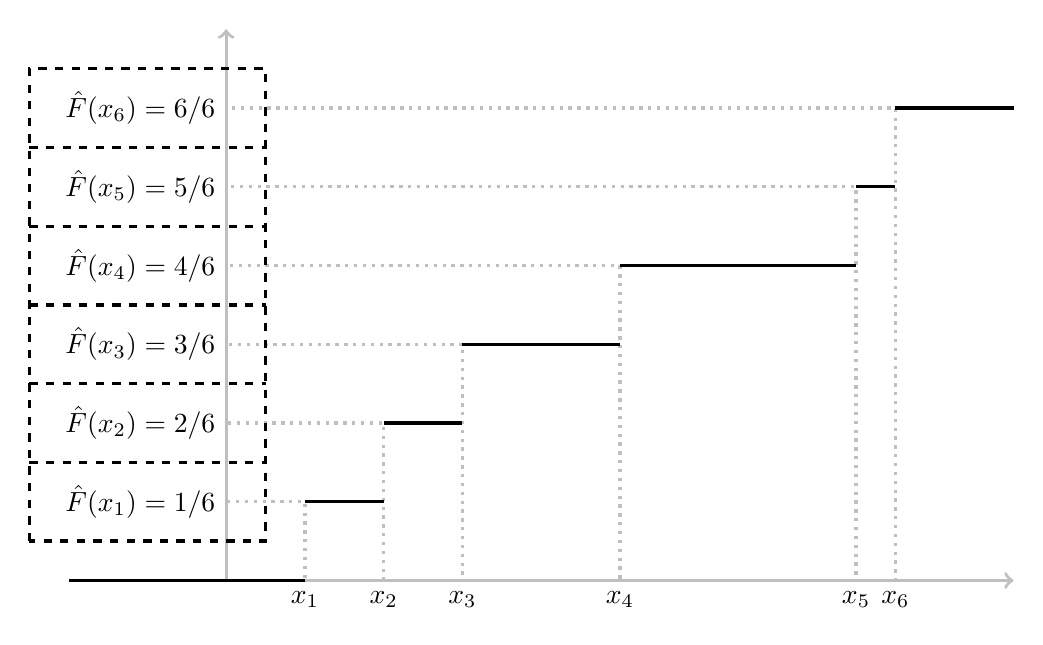
\begin{tikzpicture}[very thick]
	%\coordinate (A1) at (-5,0);
	%\coordinate (A2) at (7, 7);
	%\draw [help lines, lightgray] (A1) grid (A2);

	\newcommand*{\n}{-2.5}
	
	\foreach \x / \y in {1/1,2/2,3/3,5/4,8/5,8.5/6}{
	\node[left] (\y) at (0,\y) {$\hat{F}(x_\y) = \y/6$};
	\node[below] (\x) at (\x,0) {$x_\y$};
	\draw[dotted, lightgray] (0,0) rectangle (\x,\y);}

	\draw [<->, lightgray] (0, 7) -- (0, 0) -- (10, 0);

	%define coordinates for steps
	\coordinate (x00) at (\n + 0.5,0); \coordinate (x01) at (1,0);
	\coordinate (x10) at (1,1);\coordinate (x11) at (2,1);
	\coordinate (x20) at (2,2);\coordinate (x21) at (3,2);
	\coordinate (x30) at (3,3);\coordinate (x31) at (5,3);
	\coordinate (x40) at (5,4);\coordinate (x41) at (8,4);
	\coordinate (x50) at (8,5);\coordinate (x51) at (8.5,5);
	\coordinate (x60) at (8.5,6);\coordinate (x61) at (10,6);

	%draw stair steps (black)
	\draw (x00) -- (x01);
	\draw (x10) -- (x11);
	\draw (x20) -- (x21);
	\draw (x30) -- (x31);
	\draw (x40) -- (x41);
	\draw (x50) -- (x51);
	\draw (x60) -- (x61);

	% blue rectangles
	\draw[dashed] (\n, 0.5) rectangle (0.5,6.5);
	\foreach \x in {1.5,2.5,3.5,4.5,5.5}{
	\draw[dashed] (\n,\x) -- (0.5,\x);}

\end{tikzpicture}

\end{document}
